%Copyright (c) 2024 VOLCHOK Evgeniia

%Licensed under the Apache License, Version 2.0 (the "License");
%you may not use this file except in compliance with the License.
%You may obtain a copy of the License at

%http://www.apache.org/licenses/LICENSE-2.0


\documentclass[aspectratio=169, 18pt]{beamer}

\usepackage[english]{babel}
\usepackage{fontspec}

\usepackage{setspace}
\usepackage{pdfpages}
\usepackage{float}
\usepackage{ragged2e}
\usepackage{xcolor}
\usepackage{caption}
\usepackage{tikz}
\usetikzlibrary{positioning}
\usepackage{pifont}
\usepackage[most]{tcolorbox}
\usetheme{default}
\usepackage{graphicx}
\usepackage{amsmath,amssymb,amsfonts, mathtools}
\usepackage{cite,enumerate}
\usepackage{enumitem}
\usepackage{pgffor}
\usetikzlibrary{shadings}
\graphicspath{{figures/}}

\usepackage{minted}
\definecolor{LightGray}{gray}{0.9}
\usemintedstyle{xcode}
\usepackage{enumitem}

\usepackage{Pstyle}

\title{Presentation template}
\subtitle{Title page}

\newcommand{\insertauthorslist}{
{Speaker}, {authors}, {list}, {too  long} , {third aa} , {45345 aa}
}
	%сюда вводим списком аффиляции
\newcommand{\insertsplitinstitutes}{
{Scientific Institute 1}, {Scientific Institute 2}, {Scientific Institute 3}, {Scientific Institute 4}
}
\usepackage{enumitem}
\setlist[itemize,1]{label=$\bullet$}

%\renewcommand{labelitemii}{\textbullet}
	
\begin{document}
	
	
	\FirstFrame	
	\begin{frame}
	\titlepage
	\end{frame}
	
	\FrameStyleOne
	\begin{frame}[fragile]
		\frametitle{How to use the template: global settings}
		
		Most of style settings are in Pstyle.sty
		\begin{itemize}
			\item Use keywords and large fonts
			\item Minimum font size 20 in large auditoriums
			\item Fonts can set by \mintinline{tex}{\setmainfont{fontname}}
			\item Colours:
		\end{itemize}
			%\vspace{0.5cm}
			\centering
			\begin{tabular}{ll}
				Main blue & \textcolor{maingreen}{RGB: 0 85 34} \\
				Light blue & \textcolor{lightgreen}{RGB: 44 160 44} \\
				Purple for contrast & \textcolor{orangec}{RGB: 255 55 0} \\
			\end{tabular}
			
		\begin{itemize}
			\item Background image: 
			\begin{minted}{tex}
\usebackgroundtemplate{
\includegraphics[width=\paperwidth, height=\paperheight]
{./titlefigures/title_back.png}}
			\end{minted}
		\end{itemize}
	\end{frame}
	
	\FrameStyleTwo
	\begin{frame}[fragile]
		\frametitle{How to use the template: title page}
		\vspace{0.8cm}
		
		\begin{itemize}
		\item  Set a title and subtitle
		\begin{minted}{tex}
\title{Presentation title}
\subtitle{Title page}
		\end{minted}
		\item Authors are passed as a list in the command 
		\begin{minted}{tex}
\newcommand{\insertauthorslist}{
{Speaker}, {authors}, {list}, {too  long} , {third aa} , {45345 aa}}
		\end{minted}
		separated by comas and curly brackets surrounding each one. If the number of authors is larger than 3, only first 3 of them will be displayed with others being replaced by \textcolor{maingreen}{\textit{et. al.}}
		\item The same with affiliations
		\begin{minted}{tex}
\newcommand{\insertsplitinstitutes}{
{Scientific Institute 1}, {Scientific Institute 2},
{Scientific Institute 3}, {Scientific Institute 4}}
		\end{minted}
	\end{itemize}
		
	\end{frame}

	
	\FrameStyleThree
	\begin{frame}
		\frametitle{How to use the template: styles}
		\vspace{1cm}
		 
		Three styles for meaningful frames triggered by pre-frame commands
		
		\begin{itemize}
			\item \mintinline{tex}{\framestyleone}
			\item \mintinline{tex}{\framestyletwo}
			\item \mintinline{tex}{\framestylethree} \\
			\\
			and \\
			\item title page \mintinline{tex}{\firstframe}
			\item final page \mintinline{tex}{\thankyouframe}
		\end{itemize}
		
		\vspace{1cm}
		
		Background image and logos are in 'titlefigures' folder nested in 'figures' one.
		
		\begin{tikzpicture}[remember picture, overlay]
			
			\node [below right=-1. cm and 0.cm of current page.center]
			{
				\begin{minipage}{0.5\linewidth}
					\vspace{-0.5cm}
					
					\begin{center}
						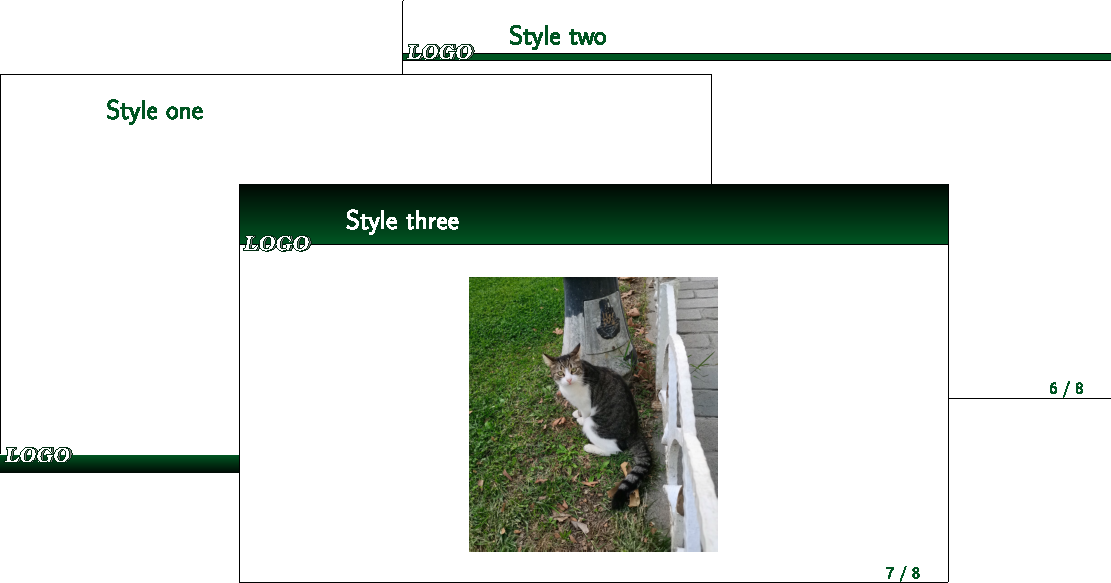
\includegraphics[width=7.cm]{styles.pdf}
					\end{center}
				\end{minipage}
			};
		\end{tikzpicture}
	\end{frame}
	
	\ThankYouFrame
	\begin{frame}
		\begin{tikzpicture}[remember picture, overlay]
			\node [below=2 cm of current page.north] (thanks)
			{
			\begin{minipage}{0.5\linewidth}
			\centering
			\LARGE\textcolor{white}{Thank you for any feedback}
			\end{minipage}
		};
			
			\node [below=1.5 cm of current page.center] (results)
			{
			\begin{minipage}{0.8\linewidth}
				\vspace{-0.5cm}
				
				\begin{center}
					
\includegraphics[width=3.cm]{./titlefigures/vibing_cat.pdf}
				\end{center}
			\end{minipage}
			};
		\end{tikzpicture}
			
	\end{frame}
	
	
	
	
	
	
\end{document}
